\documentclass{article}
% Tamaño página
\usepackage[paperheight=27cm,paperwidth=21cm,textwidth=17cm ,textheight=23cm]{geometry}
% Librería lorem ipsum?
\usepackage{lipsum}
\usepackage{fancyhdr}
\usepackage{hyperref}
\usepackage{graphicx}
\graphicspath{{images/}}
\hypersetup{
    colorlinks=true,
    linkcolor=blue,
    filecolor=magenta,      
    urlcolor=cyan,
    pdftitle={Laboratorio 1 - Hubs - Mariano Campos},
    pdfpagemode=FullScreen,
    }

\title{\bfseries \huge Laboratorio 1 - Hubs \normalsize{\linebreak\\Redes de computadoras I \\Prof.: Walter Lozano\\Prof.: Alejandro Rodriguez Costello}}
\author{\\\\\\\\\\\\Campos, Mariano Andrés \\ {\small visual.design.90@gmail.com}}
\date{\small 30 de Agosto 2024}

\begin{document}
    \maketitle
    \newpage

    \section{Conexión de 2 dispositivos}
    Realizando la configuración de dos dispositivos utilizando:
    \begin{itemize}
        \item Para la PC 1:
            \begin{itemize}
                \item Dirección de IP: 192.168.0.1
                \item Máscara de Subred: 255.255.255.0
            \end{itemize}
        \item Para la PC 2:
            \begin{itemize}
                \item Dirección de IP: 192.168.0.2
                \item Máscara de Subred: 255.255.255.0
            \end{itemize}
    \end{itemize}

    \begin{center}
        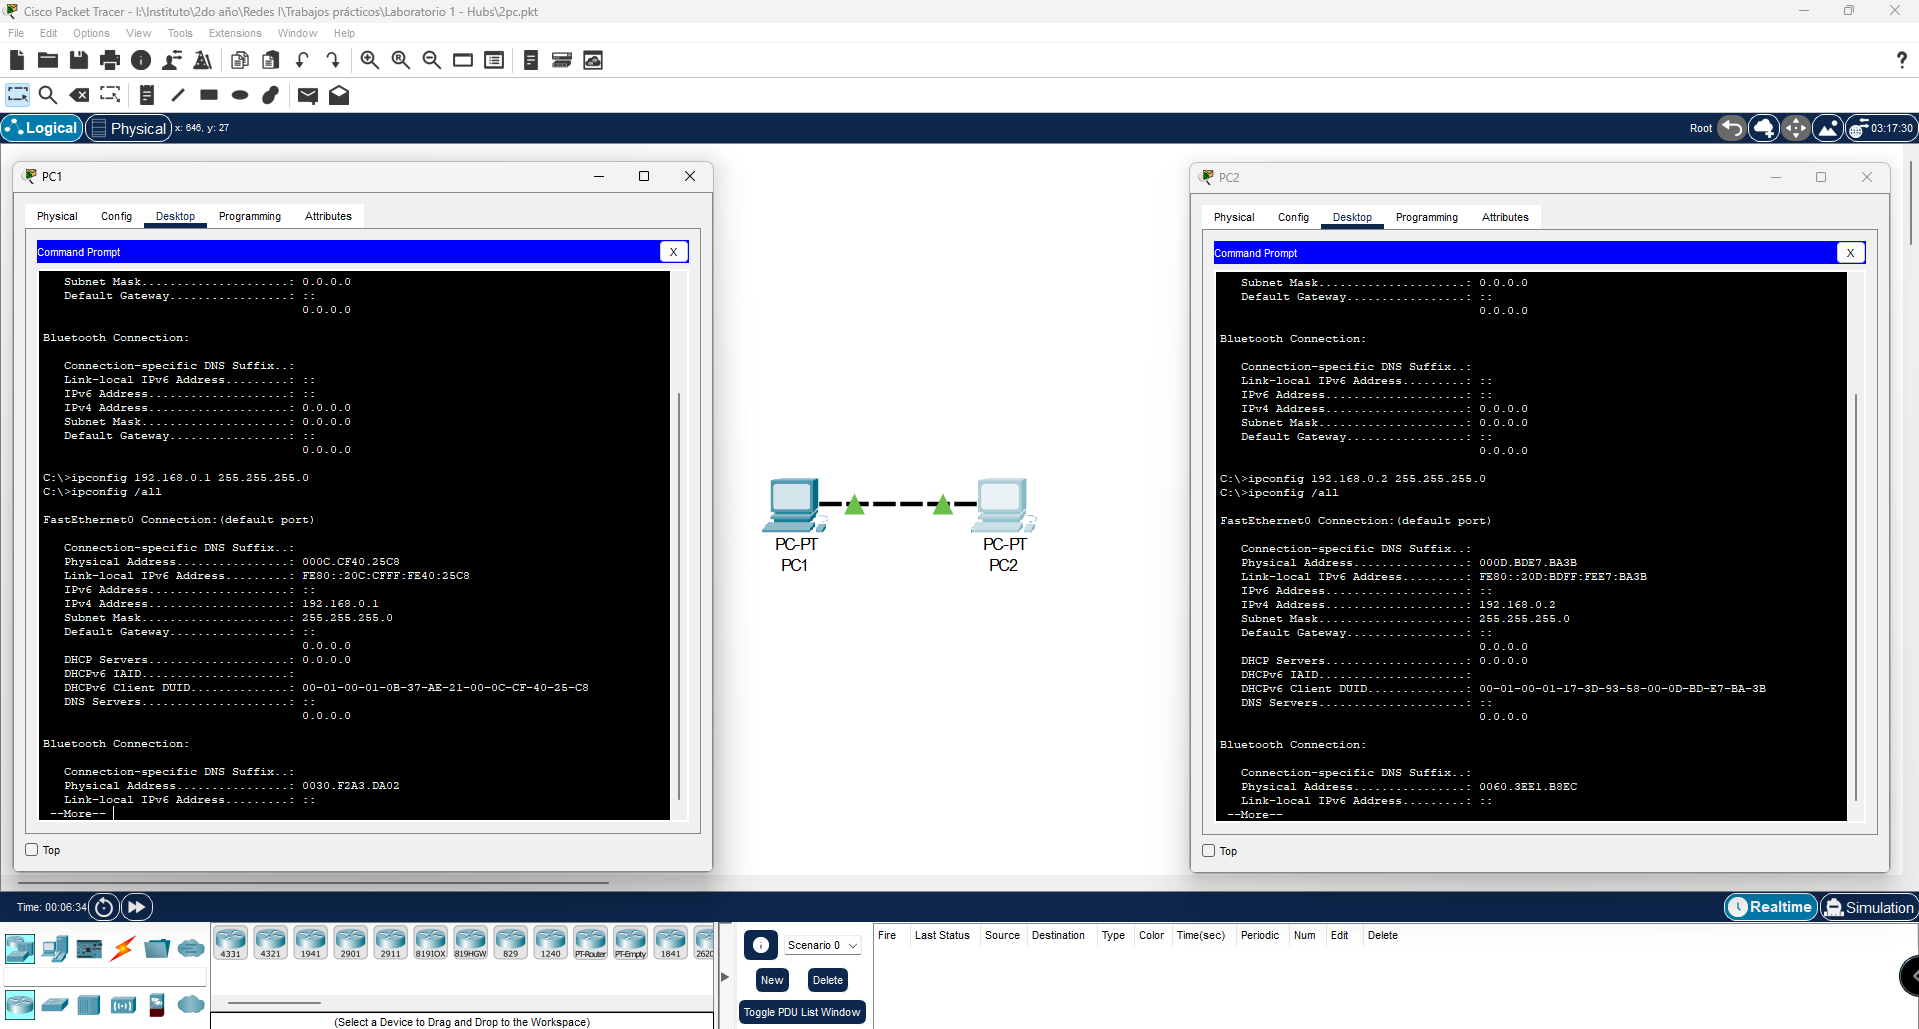
\includegraphics[width=0.65\linewidth]{img_01} 
        \linebreak
        \small {\bfseries Figura 1}: Configuración 2 computadoras.
    \end{center}

    Luego de realizar la conexión, enviamos un paquete de la PC 1 a la PC 2 utilizando el protocolo de datos PDU (Protocol Data Unit) en modo simulación:

    \begin{center}
        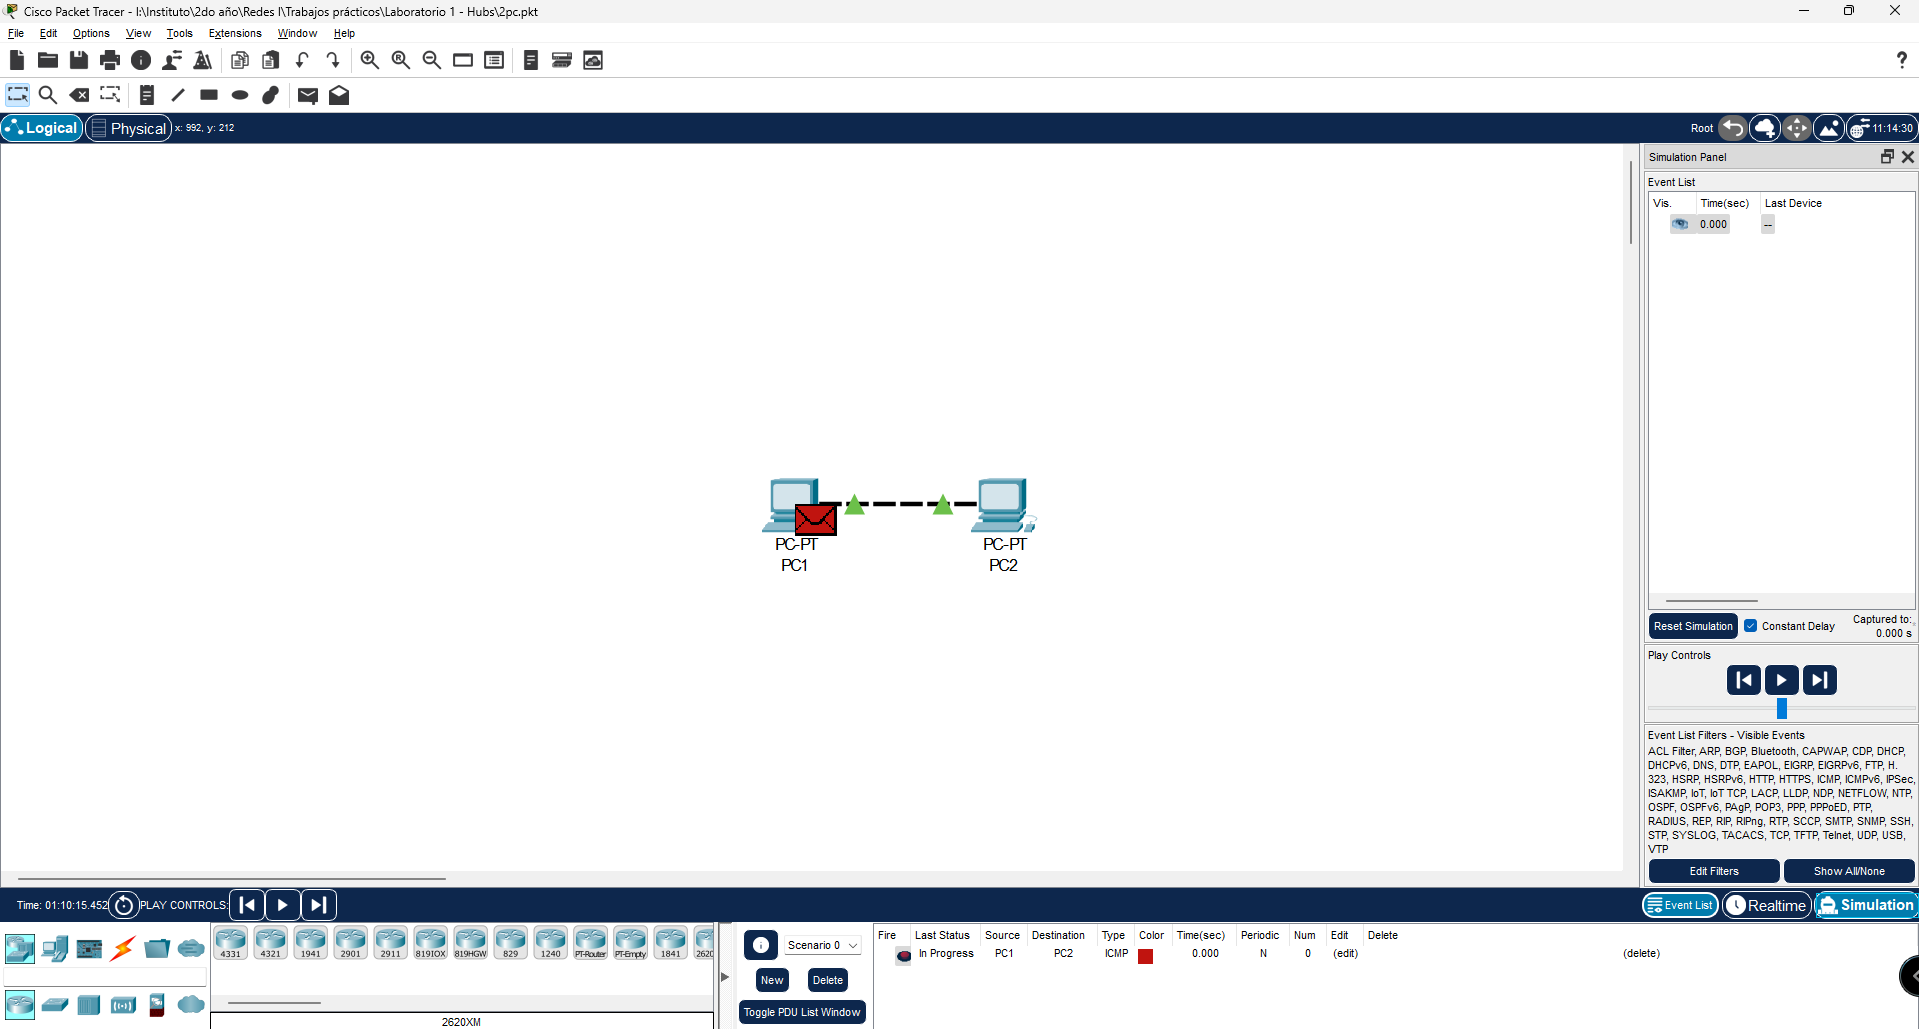
\includegraphics[width=0.45\linewidth]{img_04} 
        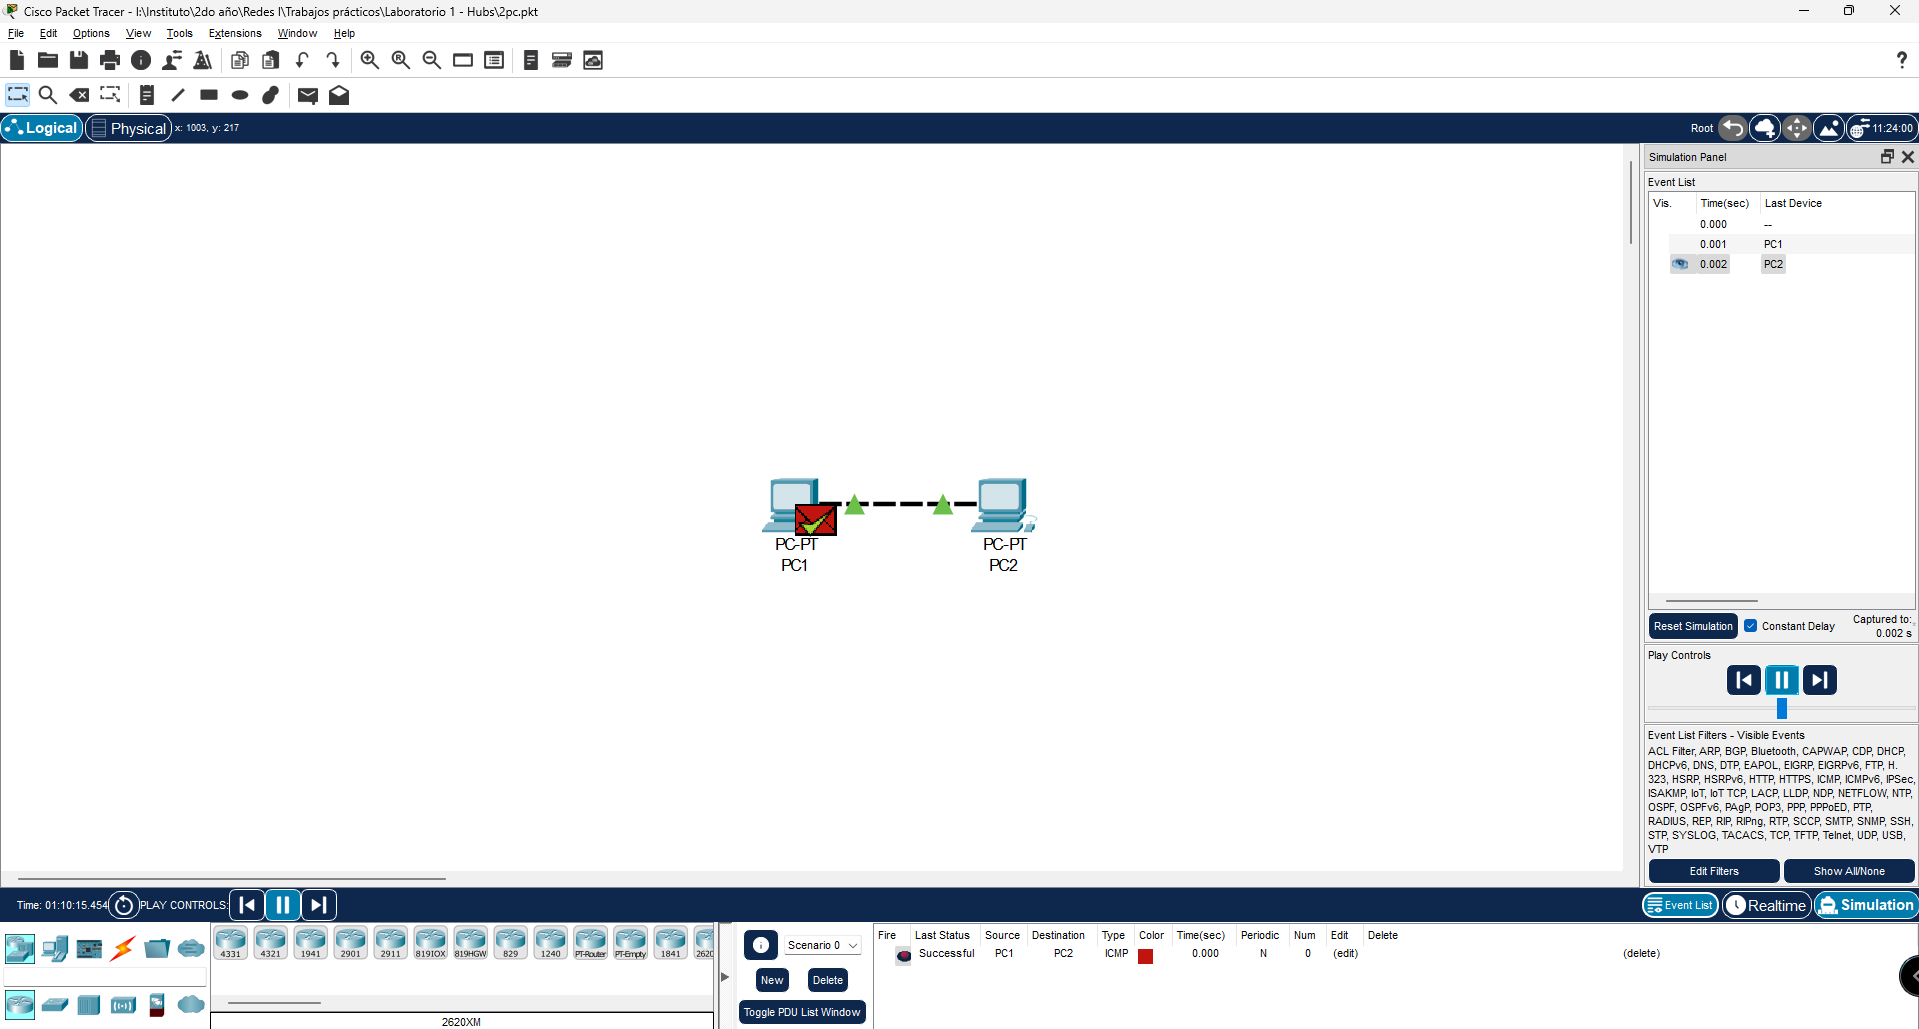
\includegraphics[width=0.45\linewidth]{img_03} 
        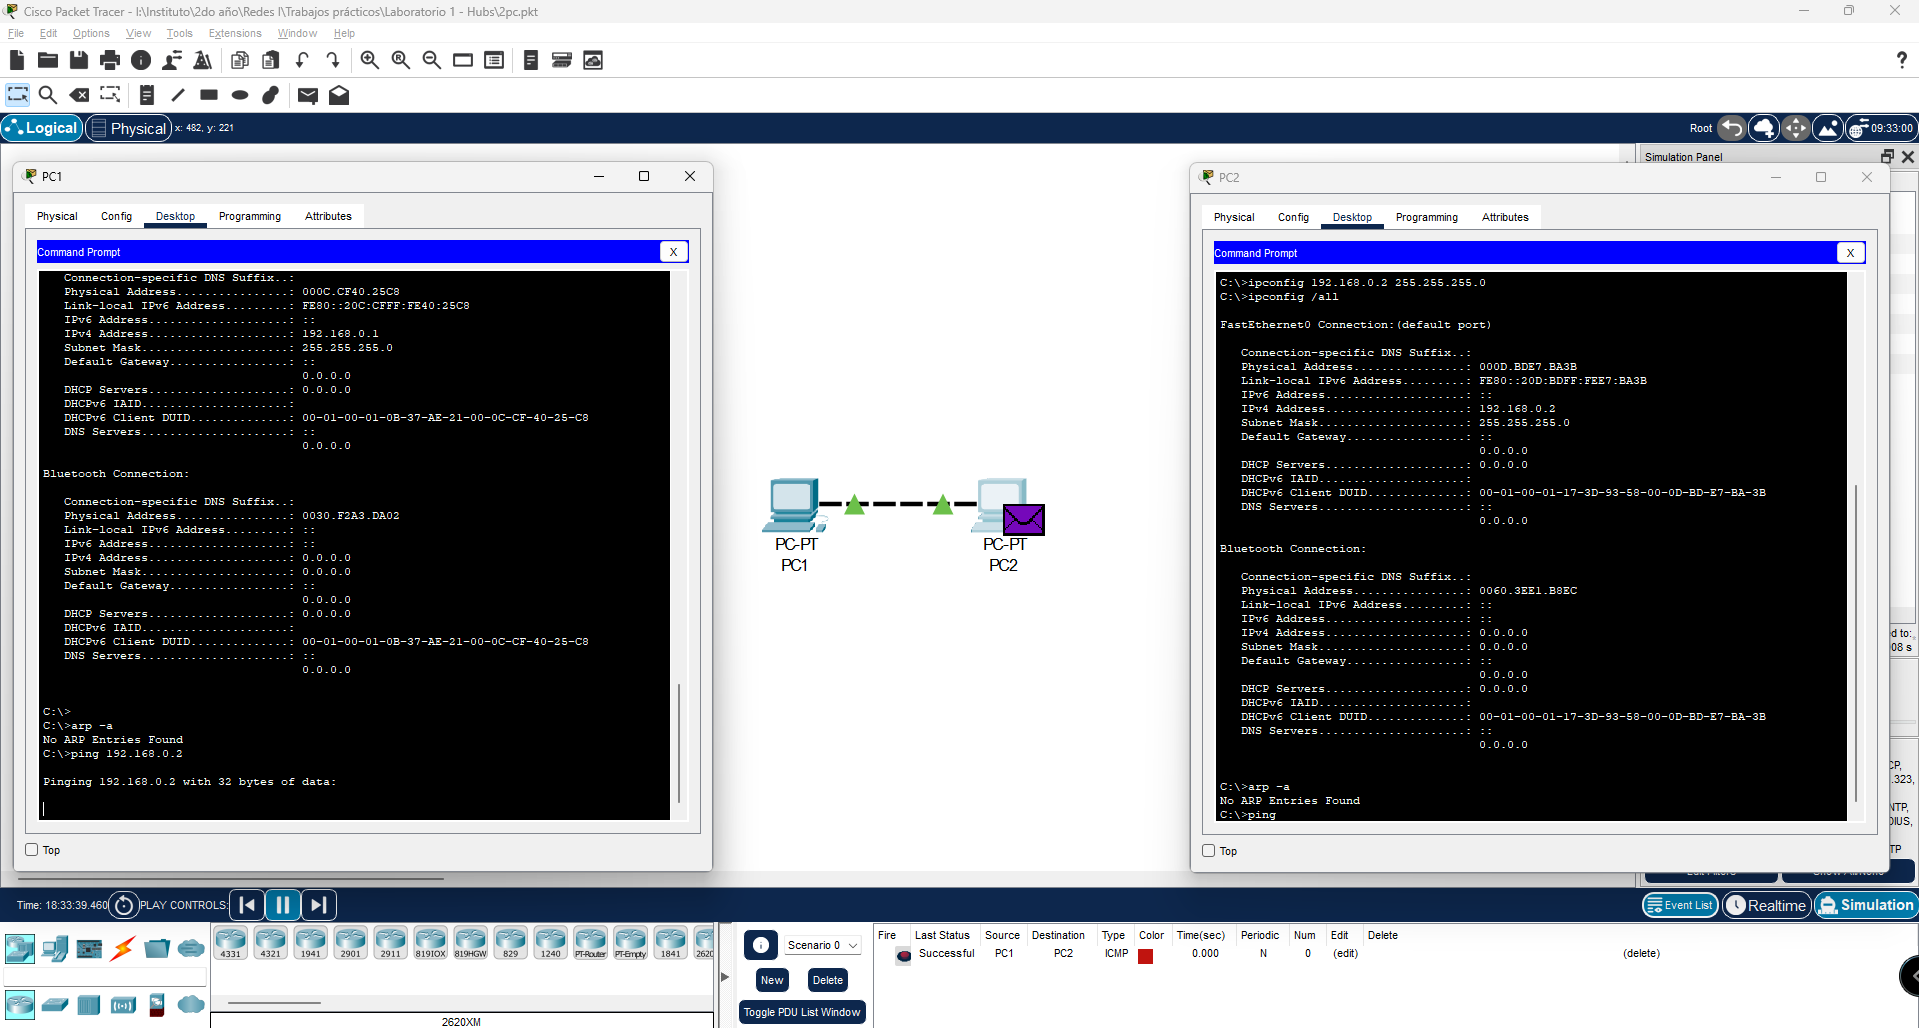
\includegraphics[width=0.45\linewidth]{img_06} 
        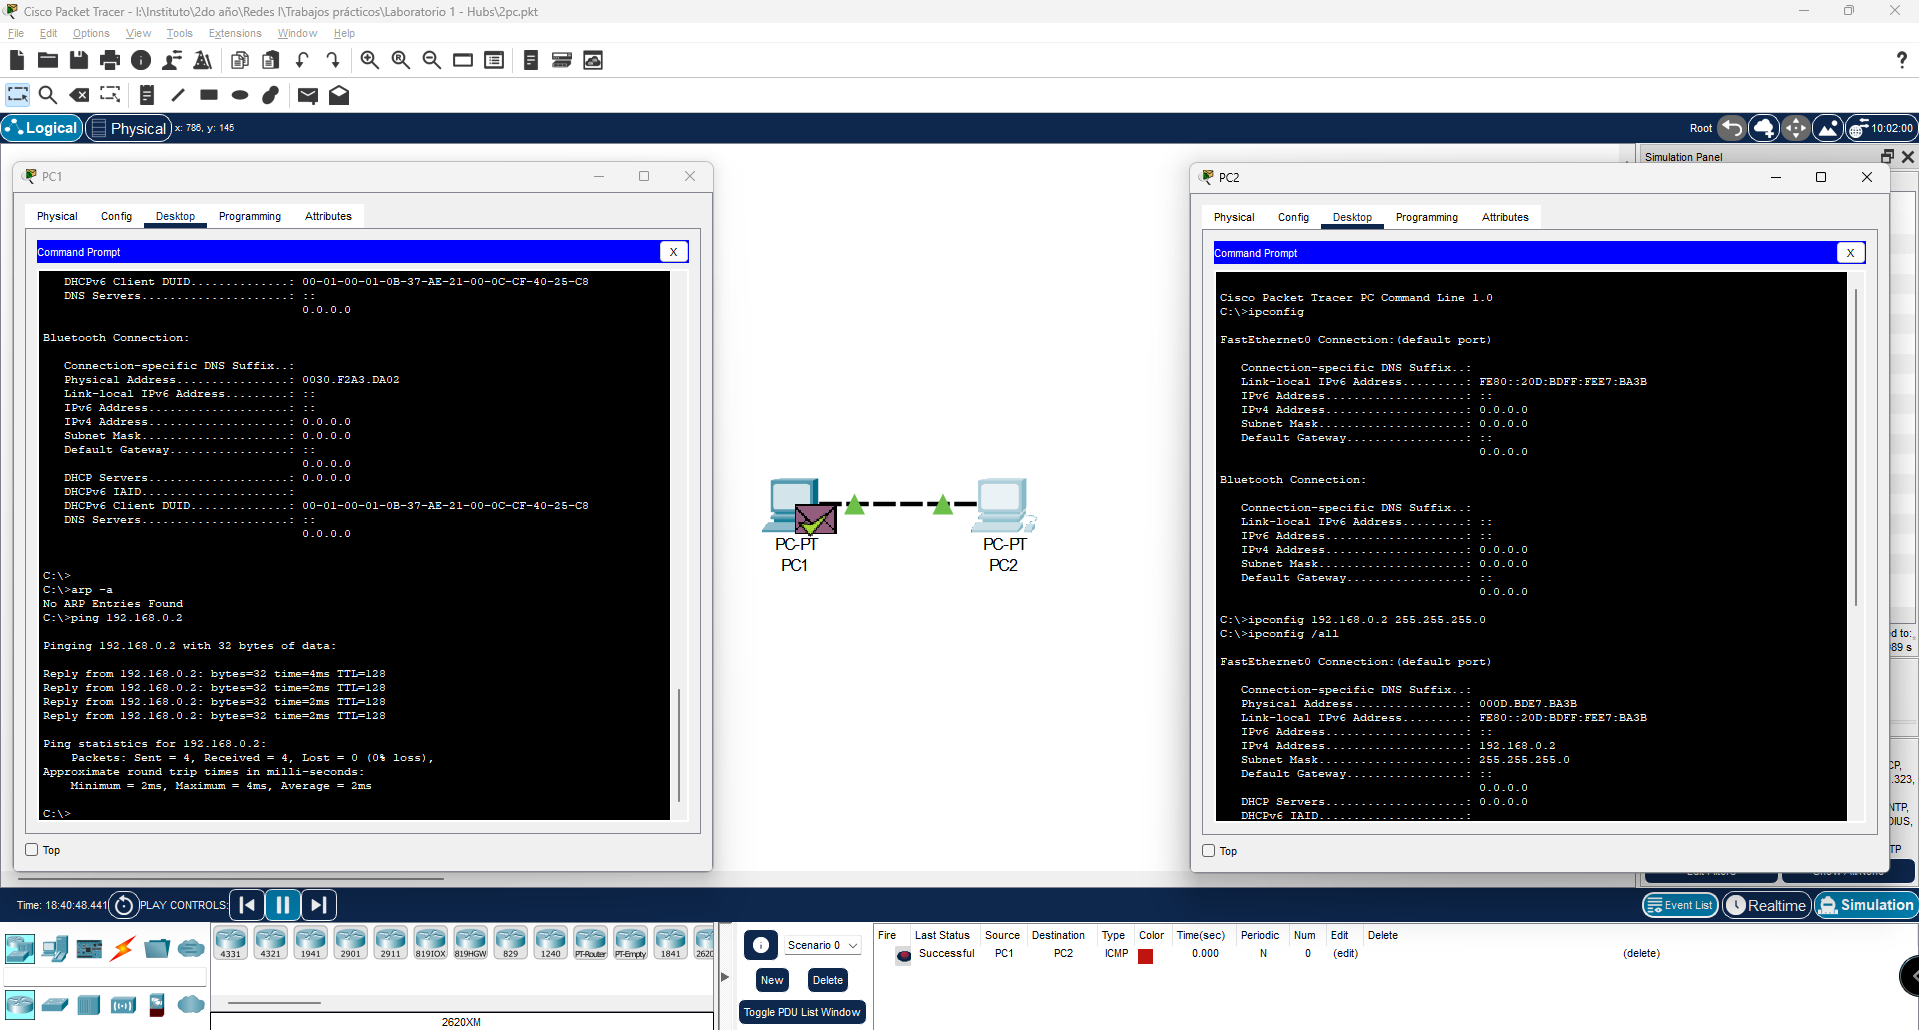
\includegraphics[width=0.45\linewidth]{img_05} 
        \linebreak
        \small {\bfseries Figura 2}: Envío y recepción de unidad de datos entre 2 PCs.
    \end{center}

    \pagebreak
    \section{Extendiendo la red}
    Para ampliar las posibilidades de una red, extenderemos la red agregando 2 pcs adicionales, conectadas mediante un hub, y el hub conectado al servidor. 

    \begin{center}
        \begin{tabular}{| p{3cm} | p{4.1cm} | p{4.1cm} | p{4.1cm} |}
            \hline
            {\bfseries N° PC} & {\bfseries Dirección MAC} & {\bfseries Dirección IP} & {\bfseries Máscara de subred} \\\hline
            PC 1 & 000C.CF40.25C8 & 192.168.0.1 & 255.255.255.0 \\\hline
            PC 2 & 0060.5C42.BDE7 & 192.168.0.2 & 255.255.255.0 \\\hline
            PC 3 & 0030.F24D.229A & 192.168.0.3 & 255.255.255.0 \\\hline
        \end{tabular}
    \end{center} 

    ¿Es necesario ir a cada dispositivo crear la tabla? - Según lo revisado en la documentación no encontré forma de acceder a la tabla de direcciones MAC de la red ni de direcciones de IP. Al parecer eso se puede hacer si tengo un Switch o un Router, a través del Command Line Interface (CLI).

    \begin{center}
        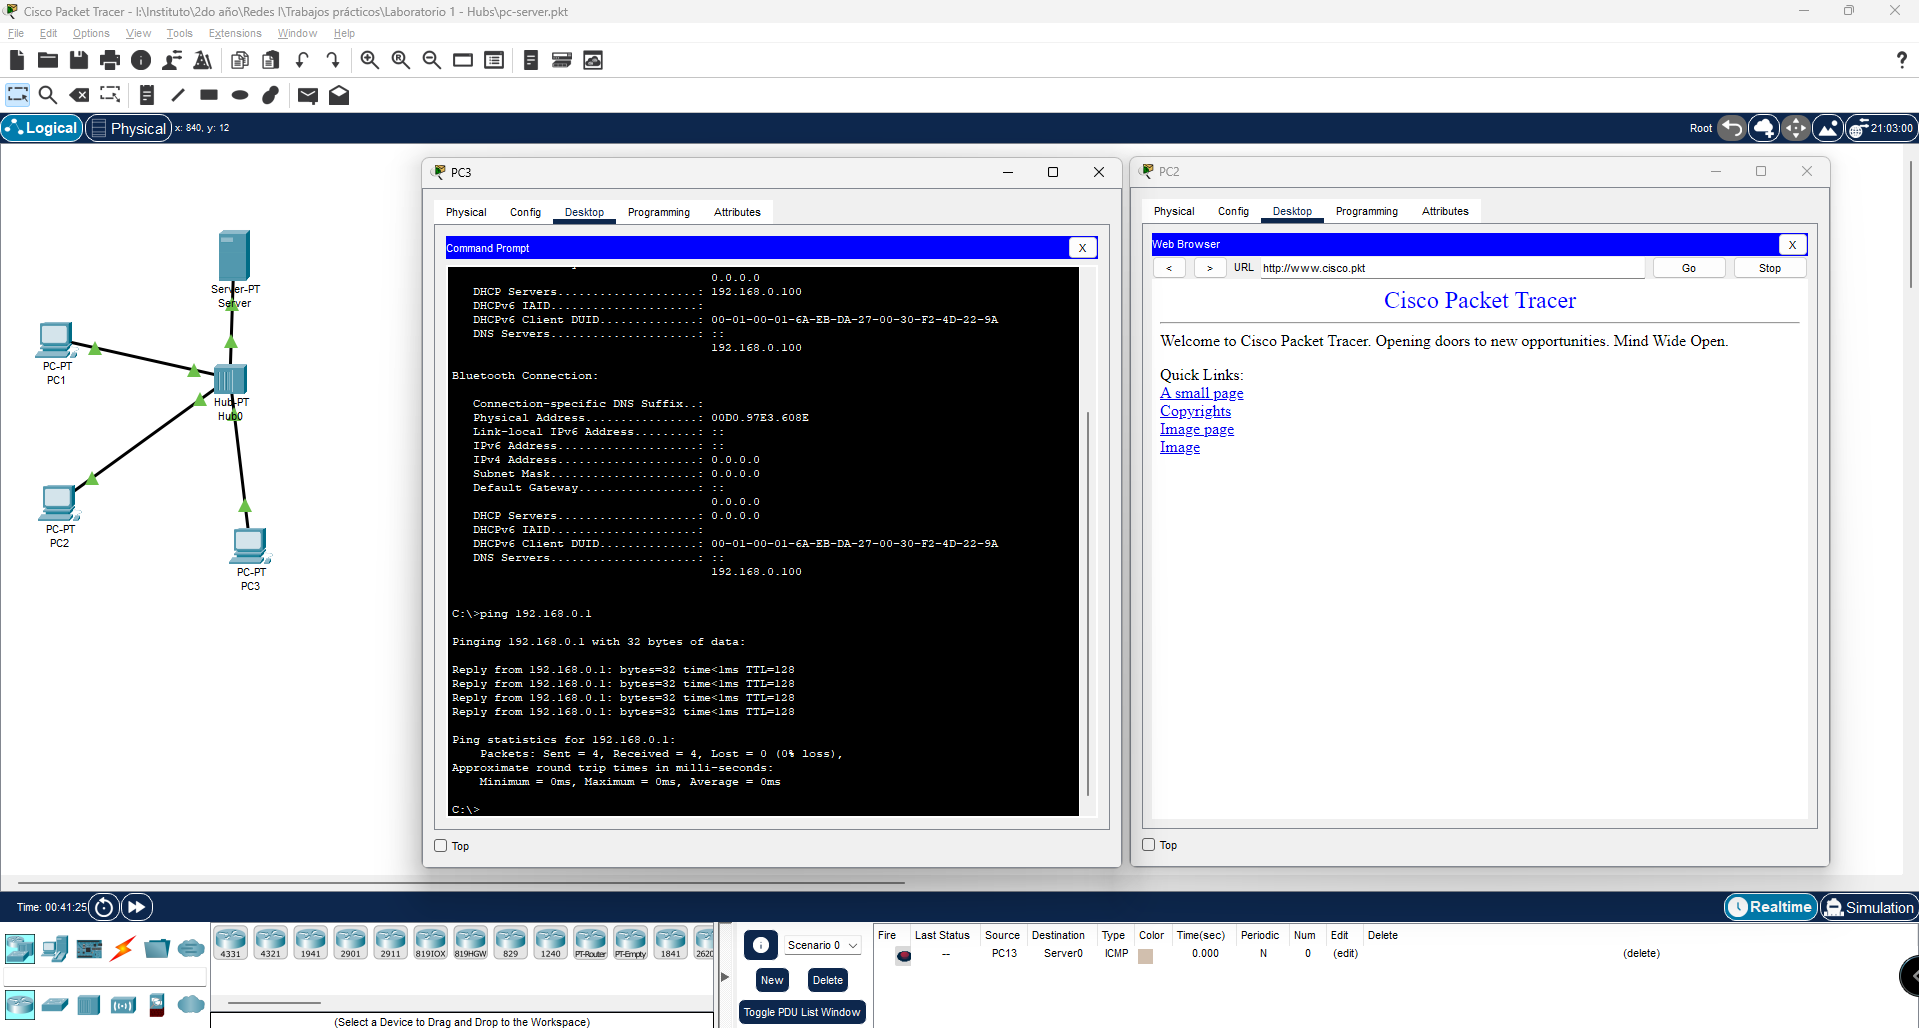
\includegraphics[width=0.85\linewidth]{img_07} 
        \linebreak
        \small {\bfseries Figura 3}: Ping entre PCs y resultado de navegación al servidor (www.cisco.pkt).
    \end{center}
    
    \pagebreak
    \section{Dominios de colisión}
    Al generar el entorno final donde conectamos una estación de ventas con 3 computadoras y una impresora a un hub, otra estación con una computadora, una impresora y 2 servidores a otro hub y un tercer hub que conecte los hub de ambas estaciones, podemos realizar la simulación donde collisionan los mensajes intentando alcanzar sus destinos.

    ¿Cuántos dominios de colisión hay? - Hay un solo dominio de colisión, la definición dice que al dominio de todos los dispositivos interconectados por el hub (en este caso) se le denomina dominio de colisión. Por lo que no importa el tamaño de la red, si las estaciones se interconectan por 1 hub, entonces tengo 1 solo dominio de colisión.
    
    \begin{center}
        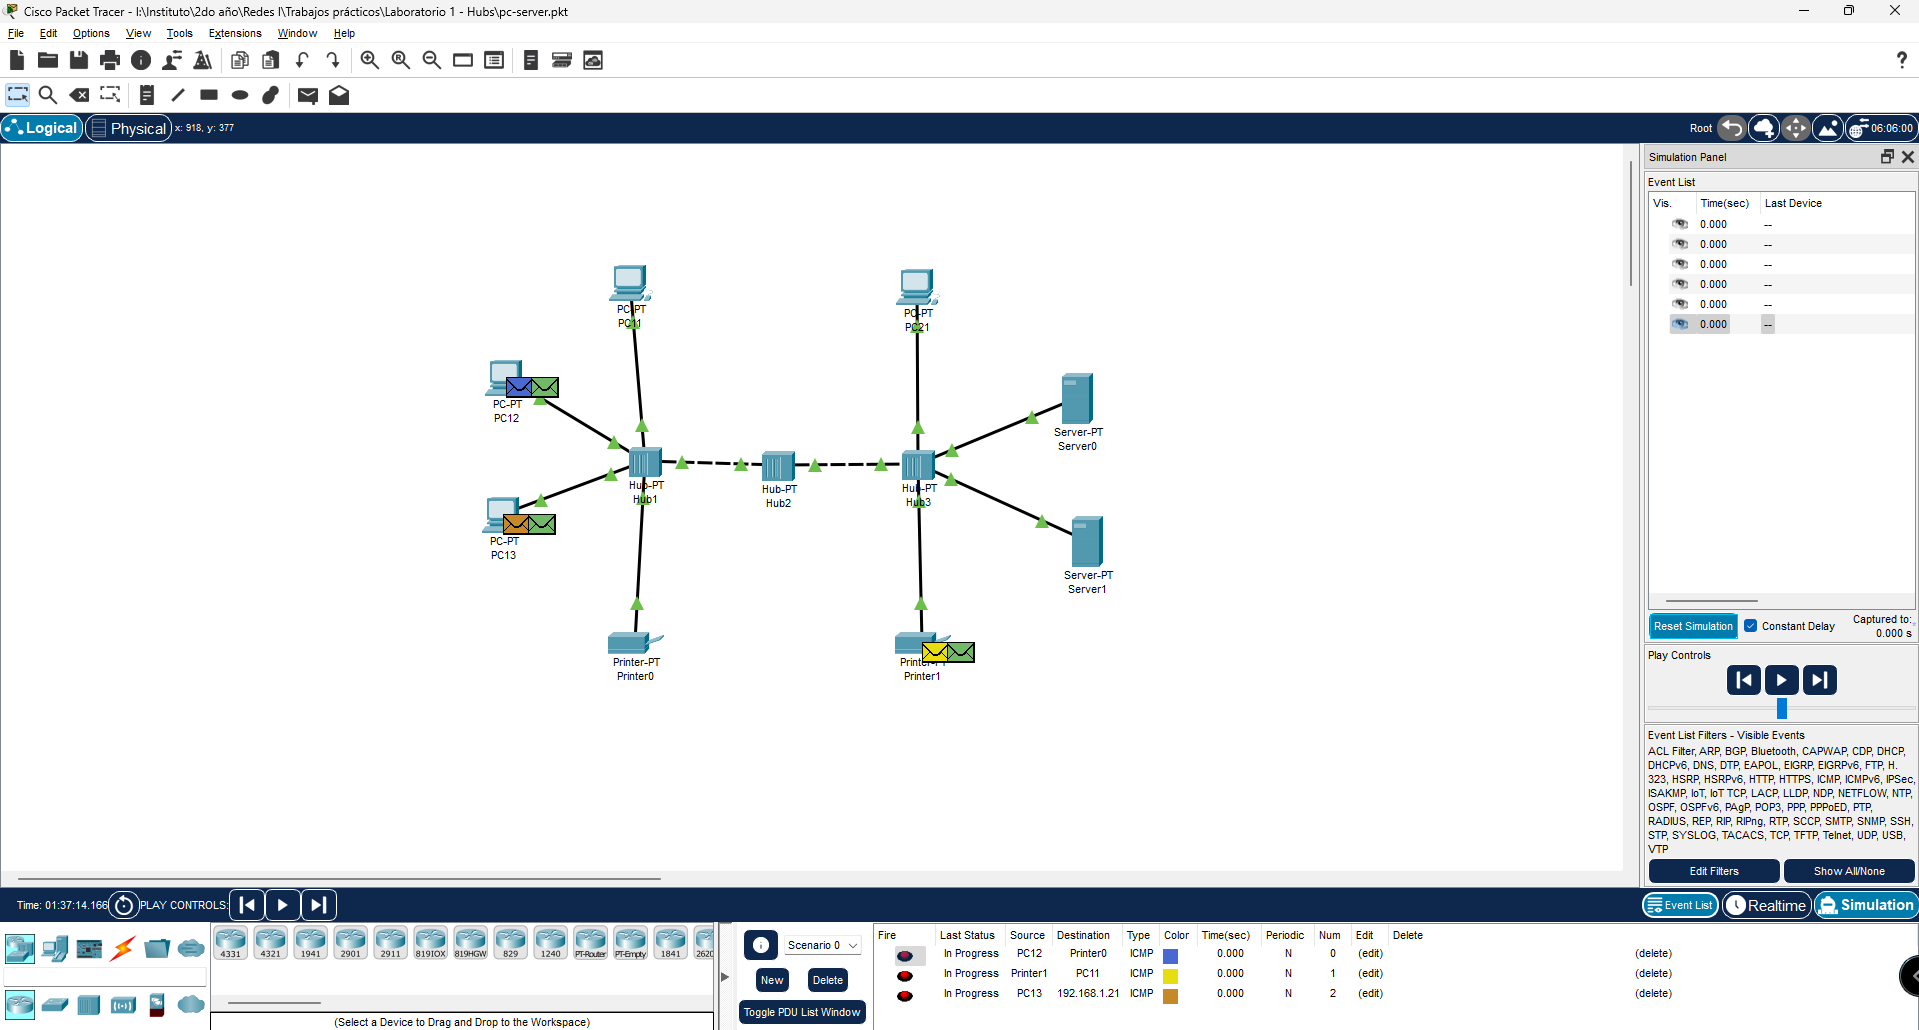
\includegraphics[width=0.45\linewidth]{img_08} 
        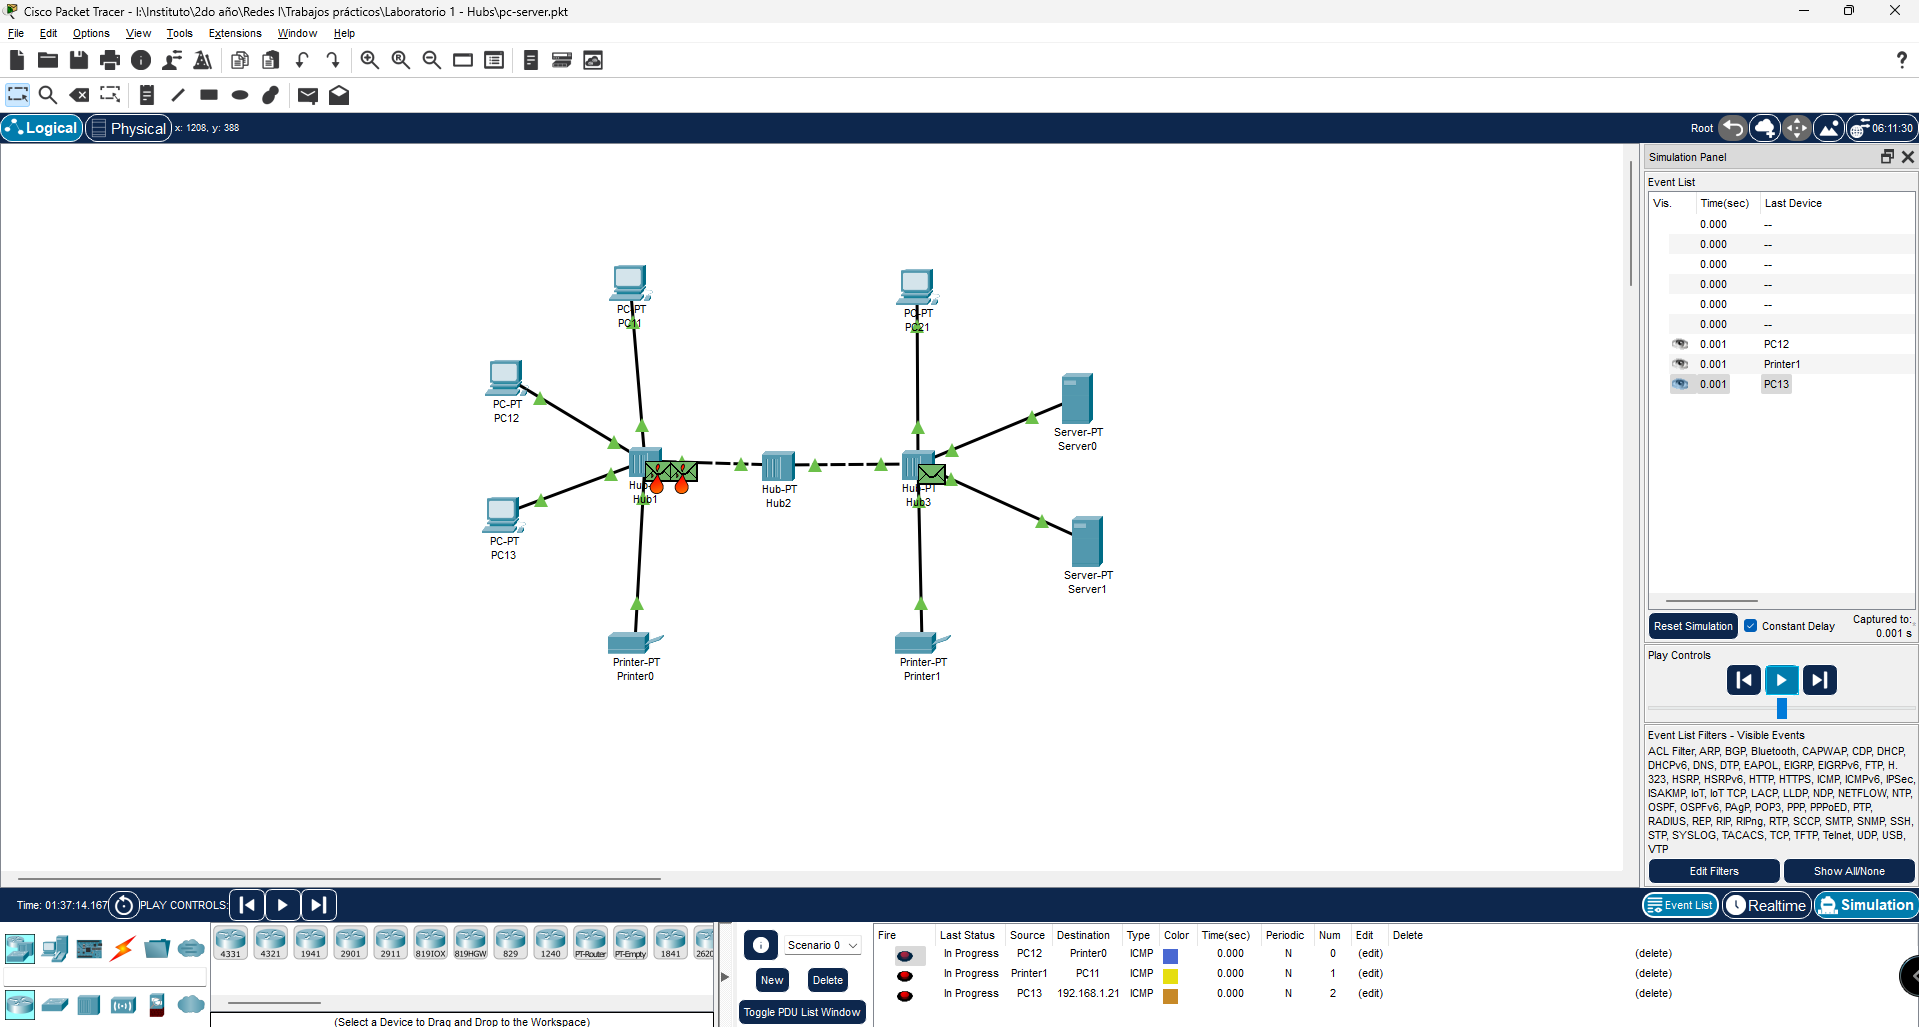
\includegraphics[width=0.45\linewidth]{img_09} 
        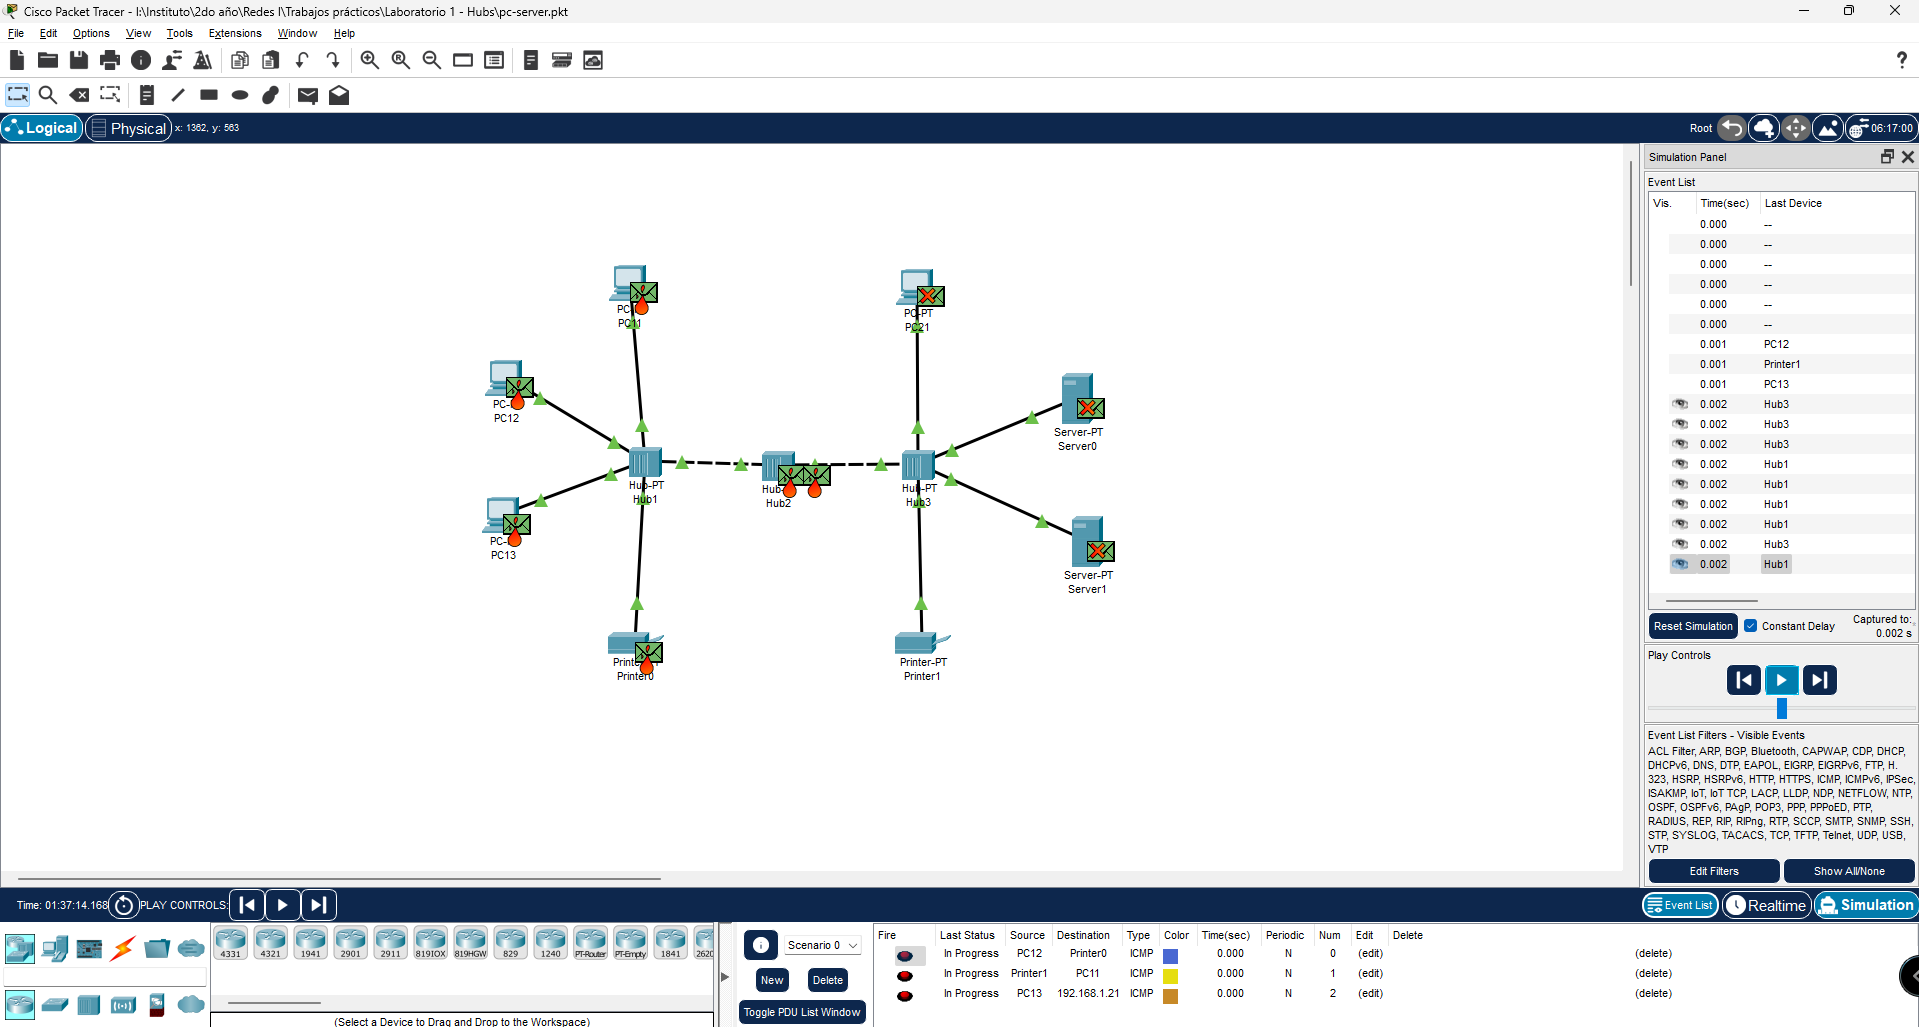
\includegraphics[width=0.45\linewidth]{img_10} 
        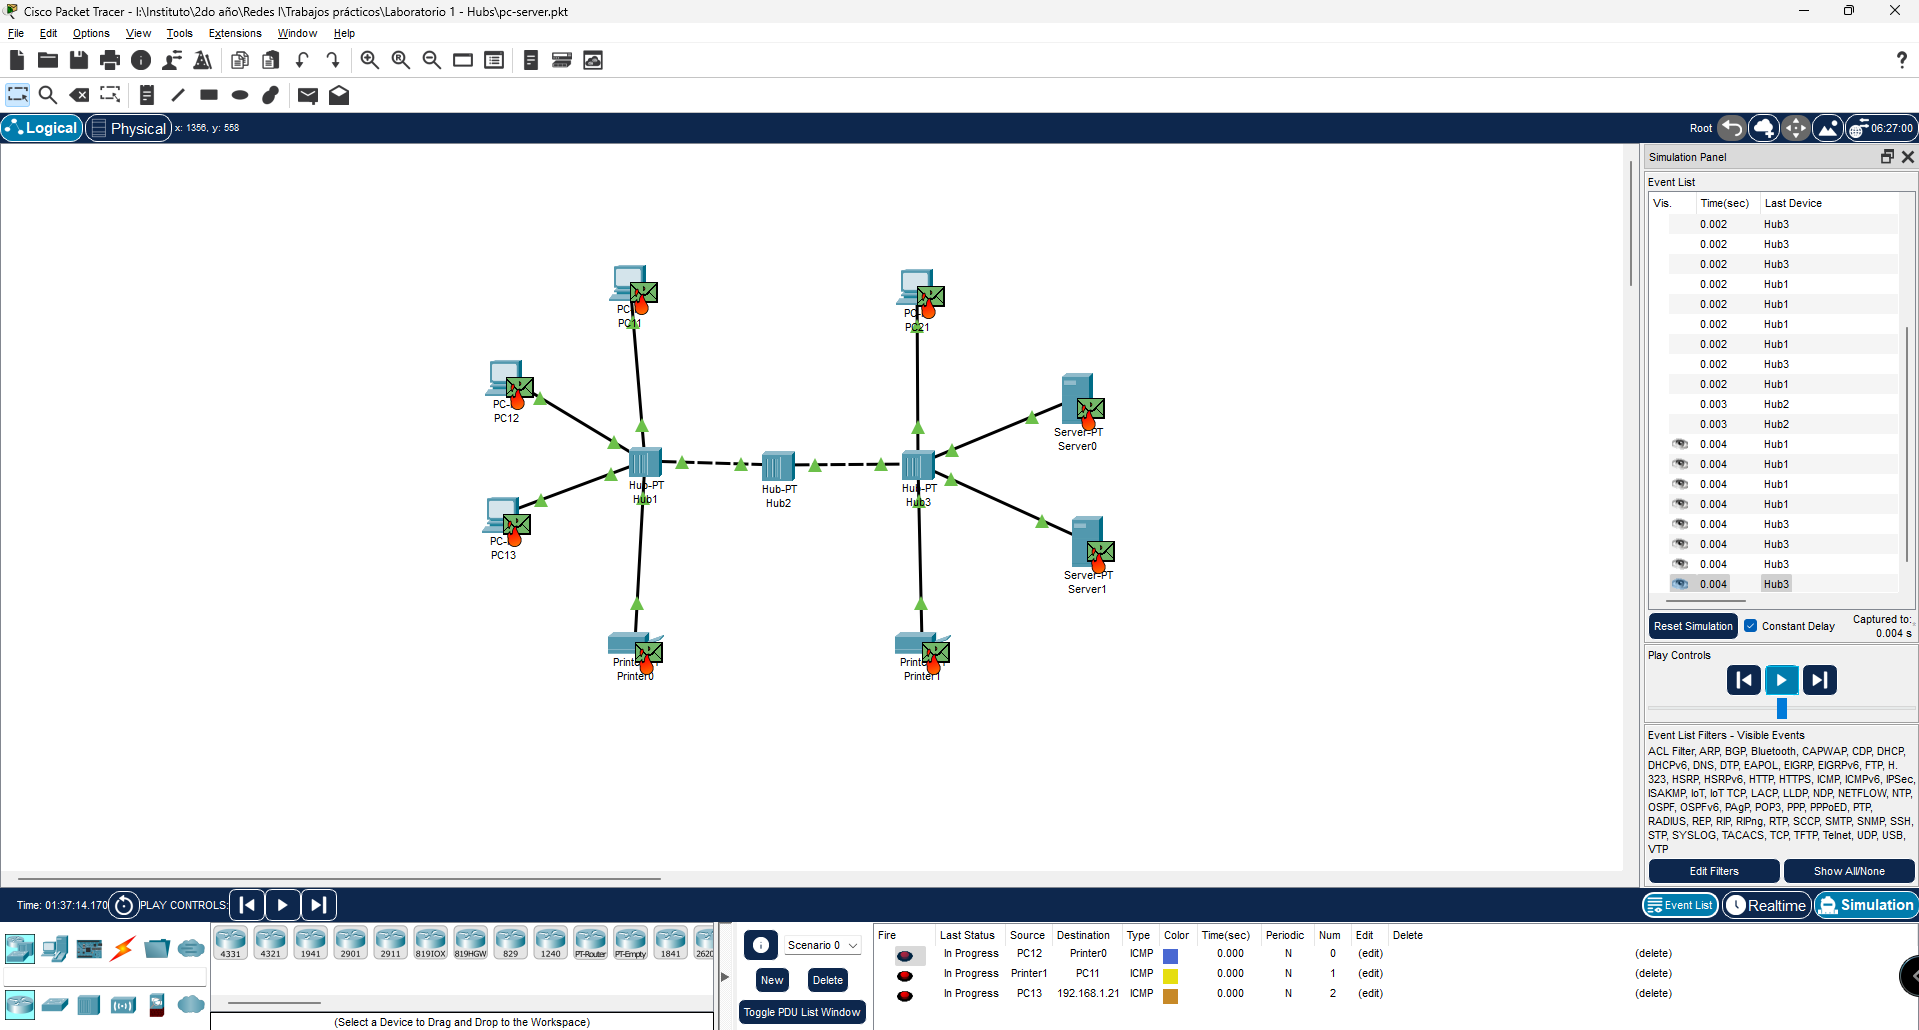
\includegraphics[width=0.45\linewidth]{img_11} 
        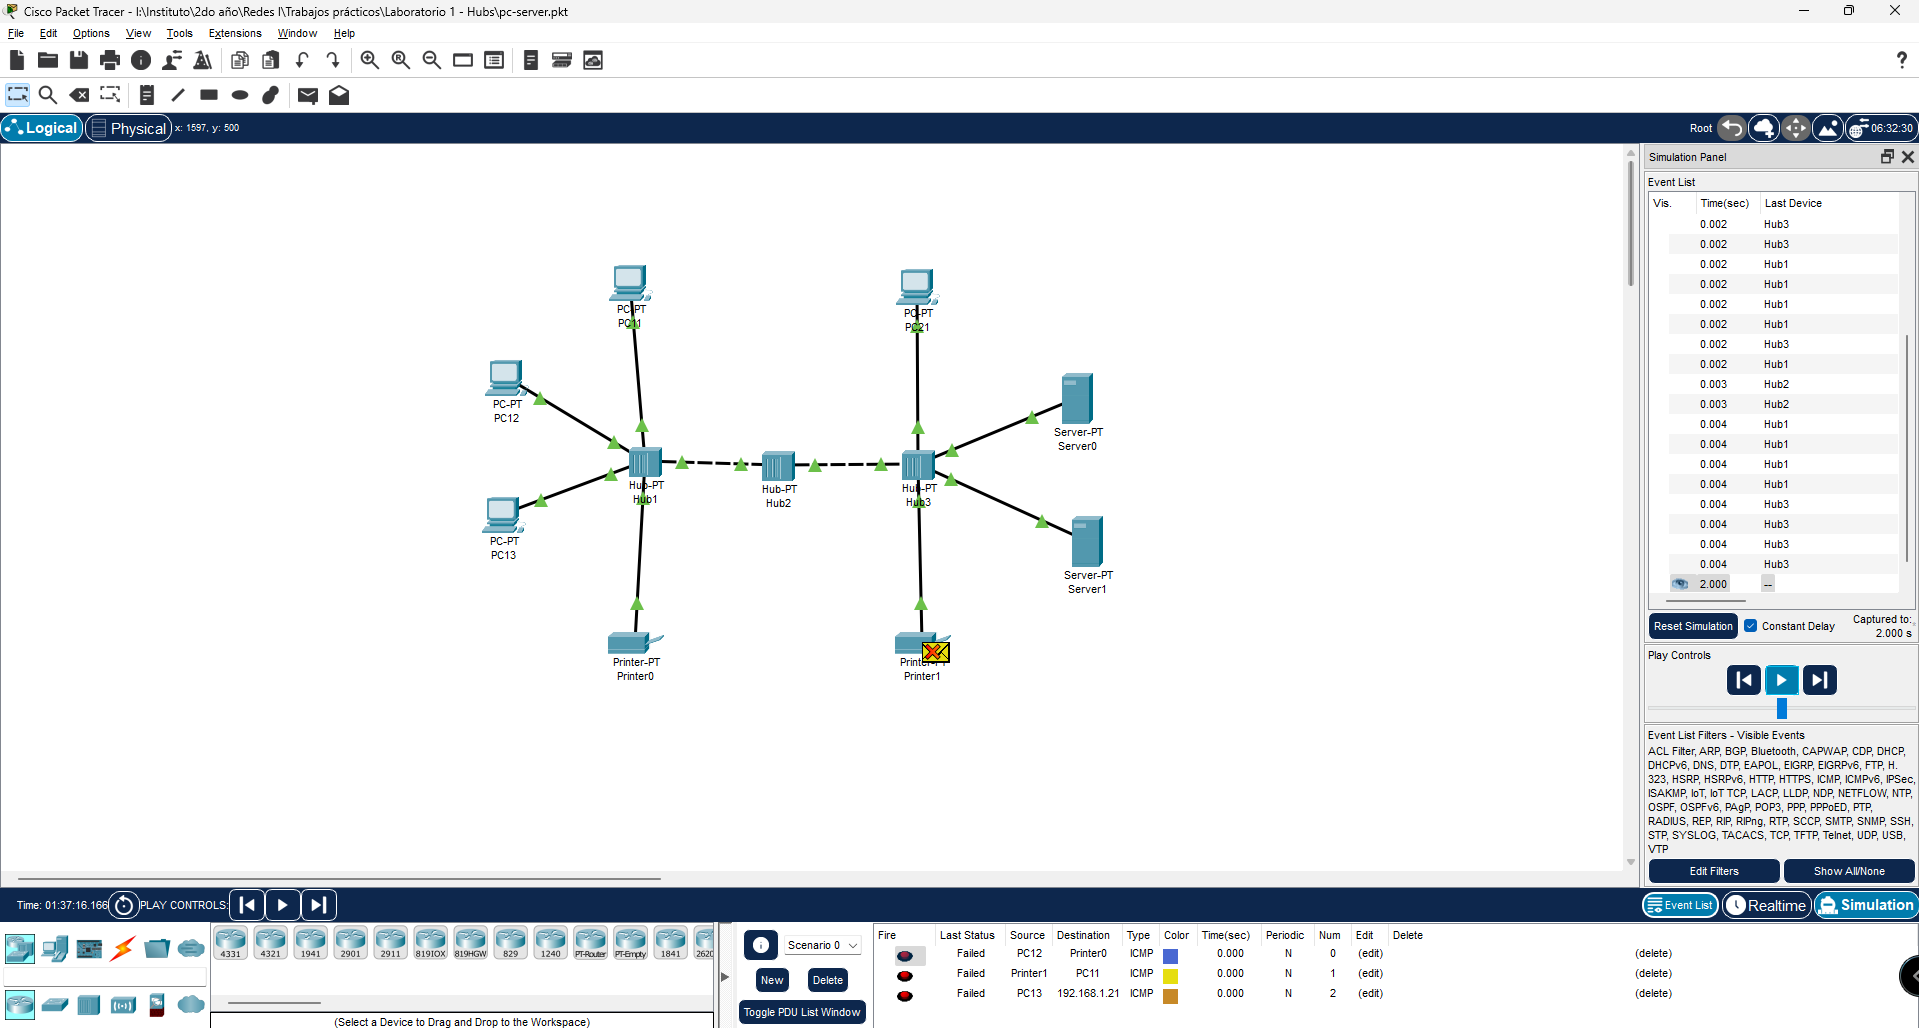
\includegraphics[width=0.45\linewidth]{img_12} 
        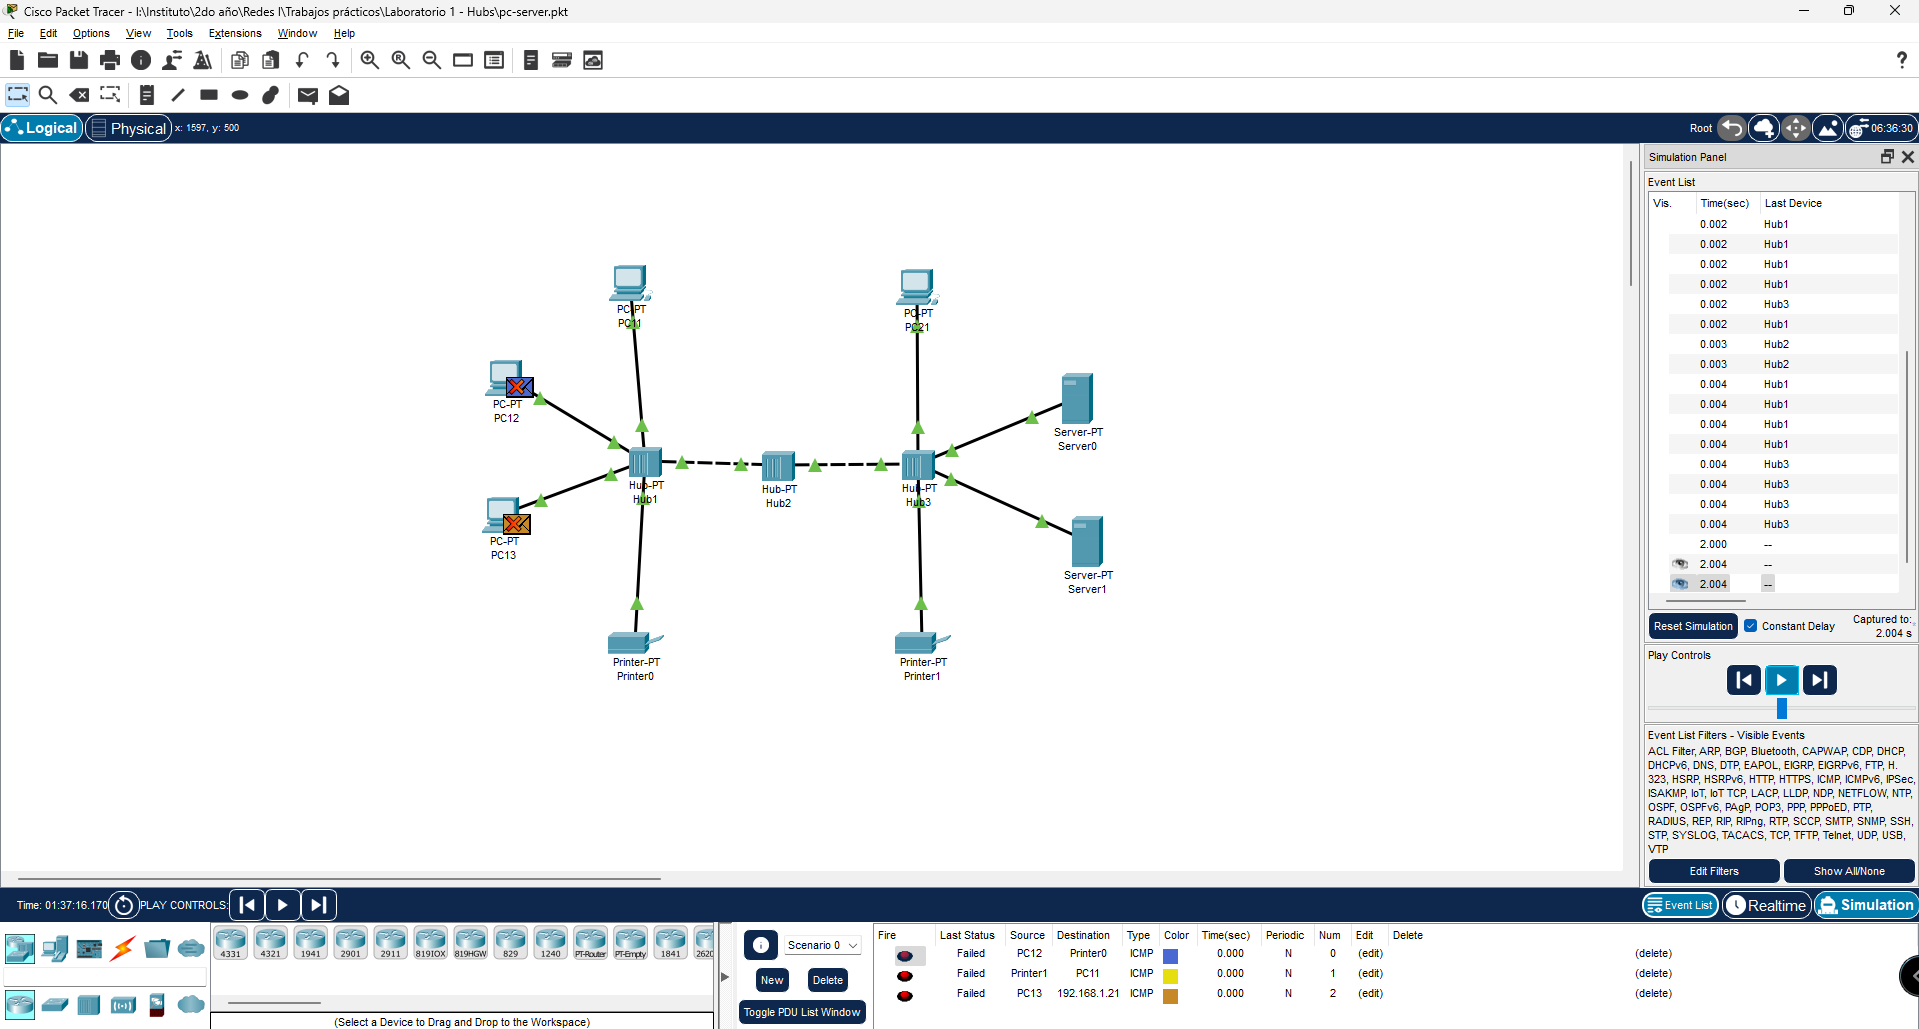
\includegraphics[width=0.45\linewidth]{img_13} 
        \linebreak
        \small {\bfseries Figura 4}: Paso a paso colisiones en escenario con múltiples hubs.
    \end{center}

    \pagebreak
    \section{Referencias}
        \begin{itemize}
            \item \href{https://github.com/MarianC312/Laboratorio_1_Hubs}{Repositorio GitHub}
            \item \href{https://www.overleaf.com/learn}{Documentación Overleaf}
            \item \href{https://community.cisco.com/t5/documentos-general/tkb-p/5761-docs-general}{Documentación General Cisco}
            \item \href{https://www.geeksforgeeks.org/how-to-configure-end-devices-on-packet-tracer/}{How to configure End Devices on Packet Tracer}
        \end{itemize}
\end{document}